%! Author = samrelins
%! Date = 04/04/2021
\scriptsize{
\begin{longtable}[c]{P{30mm}P{20mm}P{15mm}P{15mm}}
    \caption[Hospitalisation frequency and number of examples for each of the original categorical features in the ACE dataset]{Hospitalisation frequency and number of examples for each of the original categorical features in the ACE dataset. \textbf{The sample mean proportion of hospitalised patients is 0.1614}. Note that very few of the features have a proportion of hospitalised patients significantly above/below the sample mean, and those that do are supported by very few observations.}\\
    \label{tab:cat-feature-hosp-freqs}\\
    \toprule
    \textbf{Feature} & \textbf{Values} & \textbf{P(Hospital Required)} & \textbf{Total Examples} \\\toprule
    \endfirsthead
    \endhead
    \textbf{Referral From} & \textbf{CCDA} & 0.067 & 45 \\*
    & \textbf{ED} & 0.172 & 87 \\*
    & \textbf{GP} & 0.177 & 203 \\[3mm]
    \textbf{Referral Profession} & \textbf{ANP} & 0.159 & 82 \\*
    & \textbf{Consultant}  & 0.086 & 35 \\*
    & \textbf{Doctor} & 0.172 & 157 \\*
    & \textbf{Registar} & 0.177 & 62 \\[3mm]
    \textbf{Gender} & \textbf{Female} & 0.155 & 129 \\*
    & \textbf{Male} & 0.164 & 207 \\[3mm]
    \textbf{Referral Date} & \textbf{Autumn} & 0.125 & 112 \\*
    & \textbf{Spring} & 0.154 & 52 \\*
    & \textbf{Summer} & 0.169 & 59 \\*
    & \textbf{Winter} & 0.195 & 113 \\[3mm]
    \textbf{Referral Time} & \textbf{Afternoon} & 0.161 & 137 \\*
    & \textbf{Evening} & 0.4 & 15 \\*
    & \textbf{Morning} & 0.141 & 184 \\[3mm]
    \textbf{Illness Severity} & \textbf{Mild} & 0.155 & 290 \\*
    & \textbf{Moderate} & 0.205 & 44 \\[3mm]
    \textbf{Activity Level} & \textbf{Lower} & 0.188 & 112 \\*
    & \textbf{Usual} & 0.145 & 221 \\[3mm]
    \textbf{Gut Feeling} & \textbf{Low Concern} & 0.149 & 188 \\*
    & \textbf{Unwell} & 0.667 & 3 \\*
    & \textbf{Well} & 0.162 & 142 \\[3mm]
    \textbf{Sepsis} & \textbf{Low Level} & 0.158 & 19 \\*
    & \textbf{None Noted} & 0.161 & 317 \\[3mm]
    \textbf{Safeguarding} & \textbf{No} & 0.167 & 288 \\*
    & \textbf{Yes} & 0.125 & 48 \\[3mm]
    \textbf{Food Allergy} & \textbf{No} & 0.159 & 290 \\*
    & \textbf{Yes} & 0.174 & 46 \\[3mm]
    \textbf{Drug Allergy} & \textbf{No} & 0.163 & 301 \\*
    & \textbf{Yes} & 0.143 & 35 \\[3mm]
    \textbf{Other Allergy} & \textbf{No} & 0.167 & 305 \\*
    & \textbf{Yes} & 0.097 & 31 \\[3mm]
    \textbf{Group Ethnicity} & \textbf{Asian} & 0.174 & 184 \\*
    & \textbf{European} & 0.158 & 120 \\*
    & \textbf{Other} & 0.094 & 32 \\\toprule
\end{longtable}
}

\begin{table}[H]
    \centering
    \scriptsize
    \renewcommand{\arraystretch}{1.1}
    \caption[Chi$^2$ tests between categorical features and hospitalisation]{Chi$^2$ significance statistics testing the relationship between each of the original categorical features from the ACE referral data and hospitalisation outcomes. Results are ordered by p-value, lowest to highest - this can be interpreted as ``most significant'' to ``least significant''.}
    \label{tab:chi2-stats}
    \begin{tabular}{llll}
        \toprule
        & \textbf{Chi$^2$} & \textbf{p} & \textbf{dof} \\\toprule
        \textbf{Referral Time} & 6.881 & 0.032 & 2 \\
        \textbf{Gut Feeling} & 5.929 & 0.052 & 2 \\
        \textbf{Referral From} & 3.446 & 0.179 & 2 \\
        \textbf{Activity Level} & 0.719 & 0.397 & 1 \\
        \textbf{Other Allergy} & 0.579 & 0.447 & 1 \\
        \textbf{Group Ethnicity} & 1.307 & 0.52 & 2 \\
        \textbf{Illness Severity} & 0.371 & 0.542 & 1 \\
        \textbf{Referral Date} & 2.078 & 0.556 & 3 \\
        \textbf{Safeguarding} & 0.266 & 0.606 & 1 \\
        \textbf{Referral Profession} & 1.738 & 0.628 & 3 \\
        \textbf{Sepsis} & 0.082 & 0.774 & 1 \\
        \textbf{Gender} & 0.005 & 0.943 & 1 \\
        \textbf{Drug Allergy} & 0.004 & 0.952 & 1 \\
        \textbf{Food Allergy} & 0.002 & 0.963 & 1 \\\toprule
    \end{tabular}
\end{table}

\begin{figure}[H]
    \caption[Box and KDE plots of numerical features]{Box plots (left) and stacked KDE plots (right) for each of the numerical features, grouped by examples that required hospital treatment and those that were successfully discharged from ACE. The stacked KDE plots maintain the original proportions of patients that were referred to hospital / successfully discharged from ACE and serve as a good indicator of the proportions of examples that represent the numeric features at different values.}
    \label{fig:num-features-dist}
    \centering
    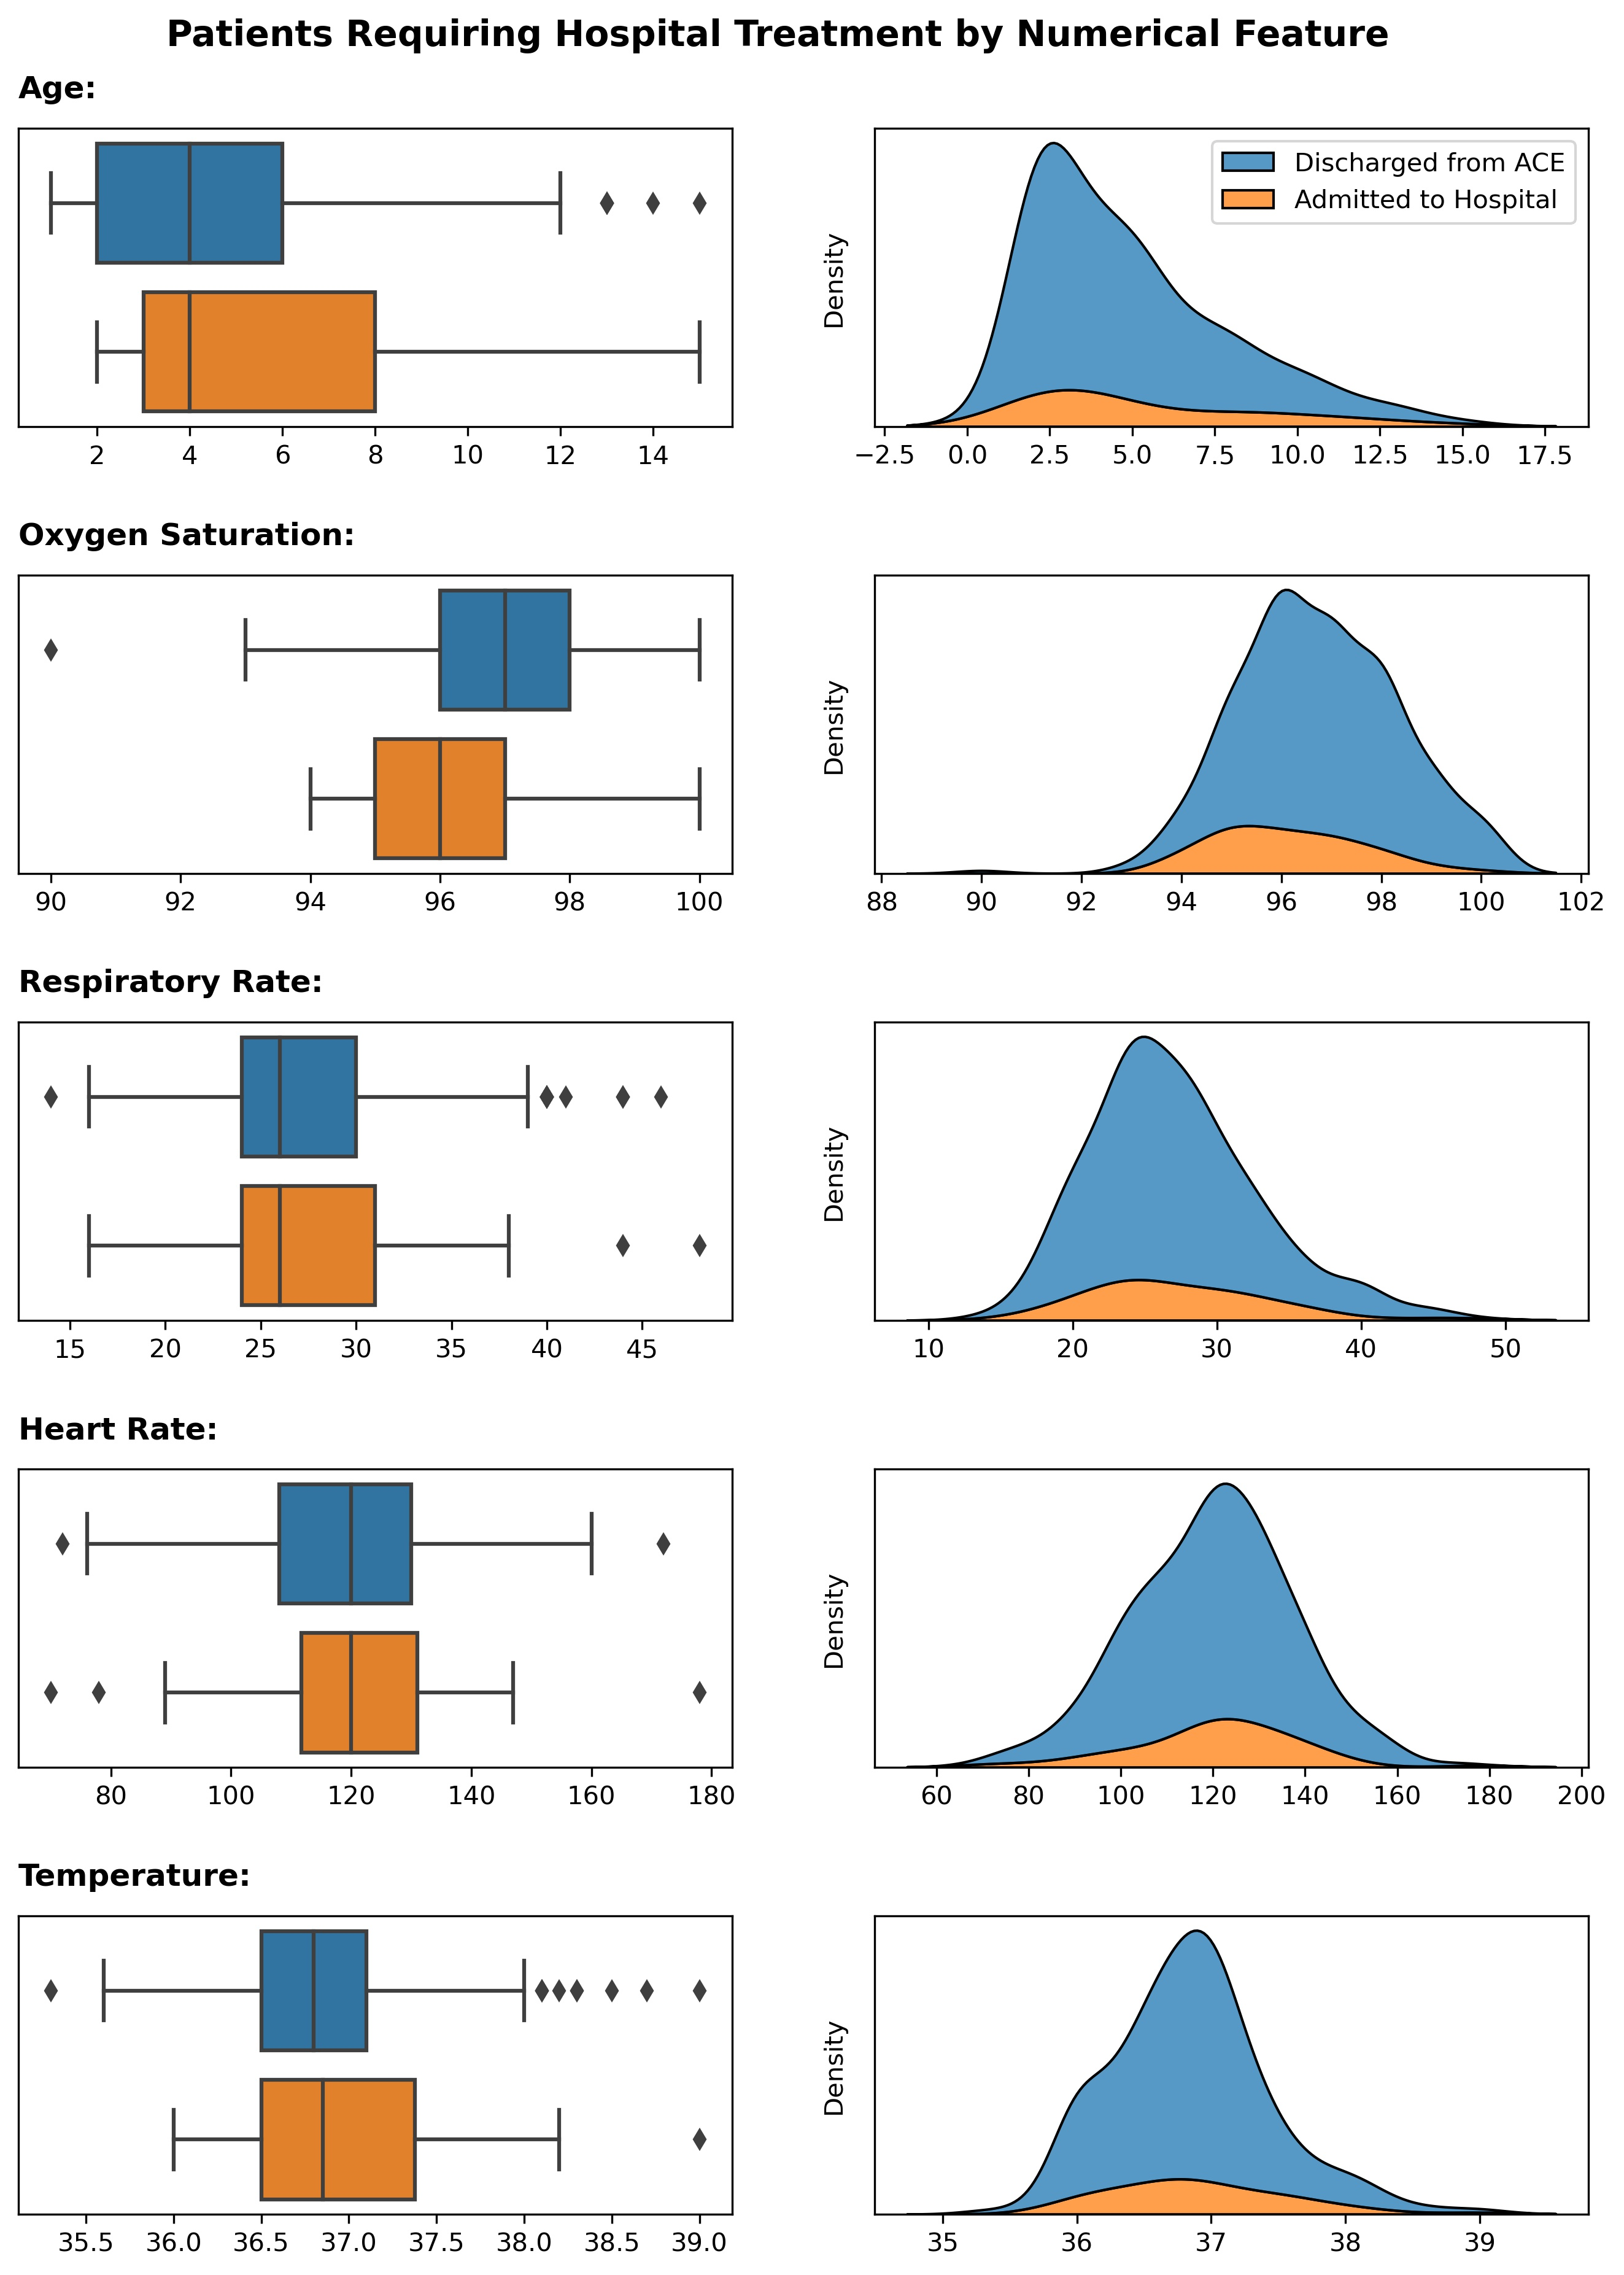
\includegraphics[width=1\textwidth]{num-features-dist}
\end{figure}

\begin{table}[H]
    \scriptsize
    \centering
    \renewcommand{\arraystretch}{1.1}
    \caption[Pearson's R statistics for the numeric/continuous features in the ACE referral data]{Pearson's R statistics for the numeric/continuous features in the ACE referral data. The high statistical significance of the Oxygen Saturation feature can be seen in \Cref{fig:num-features-dist}. The proportions of patients hospitalised/discharged change significantly at either tail of the distribution - the lower tail has a much greater proportion of patients hospitalised and the opposite for the higher tail. It should be noted that the bulk of the examples lie in the center of the distribution and don't exhibit high or low oxygen saturations.}
    \label{tab:pearsons-stats}
    \begin{tabular}{lll}
        \toprule
                             & \textbf{r} & \textbf{p} \\\toprule
        \textbf{Oxygen Saturation}      & -0.164     & 0.003      \\
        \textbf{Age}         & 0.081      & 0.141      \\
        \textbf{Temperature}        & 0.048      & 0.409      \\
        \textbf{Respiratory Rate}   & 0.028      & 0.617      \\
        \textbf{Heart Rate}  & 0.017      & 0.752\\\toprule
    \end{tabular}
\end{table}

\begin{table}[H]
    \scriptsize
    \centering
    \caption[Features from ACE referral criteria and APLS observation guidelines]{Hospitalisation Frequency and number of examples for each of the features engineered using the ACE referral criteria and APLS observation guidelines}
    \label{tab:extra-feature-hosp-freqs}
    \begin{tabular}{P{30mm}P{20mm}P{15mm}P{15mm}}
        \toprule
        \textbf{Feature} & \textbf{Values} & \textbf{P(Hospital Required)} & \textbf{Total Examples} \\\toprule
        \textbf{APLS Resp Rate} & \textbf{High} & 0.207 & 82 \\*
        & \textbf{Low} & 0.0 & 4 \\*
        & \textbf{Normal} & 0.148 & 250 \\[3mm]
        \textbf{APLS Heart Rate} & \textbf{High} & 0.242 & 33 \\*
        & \textbf{Low} & 0.5 & 2 \\*
        & \textbf{Normal} & 0.15 & 301 \\[3mm]
        \textbf{Ox Sat Low} & \textbf{No} & 0.162 & 333 \\*
        & \textbf{Yes} & 0.0 & 3 \\[3mm]
        \textbf{Age Range} & \textbf{Pre School} & 0.161 & 180 \\*
        & \textbf{Primary} & 0.141 & 142 \\*
        & \textbf{Secondary} & 0.357 & 14 \\[3mm]
        \textbf{ACE Heart Rate}  & \textbf{high} & 0.154 & 65 \\*
        & \textbf{Low} & 0.286 & 7 \\*
        & \textbf{Normal} & 0.159 & 264 \\[3mm]
        \textbf{ACE Resp Rate} & \textbf{high} & 0.17 & 112 \\*
        & \textbf{Low} & 0.175 & 40 \\*
        & \textbf{Normal} & 0.152 & 184 \\[3mm]
        \textbf{Meets ACE Criteria} & \textbf{No} & 0.17 & 182 \\*
        & \textbf{Yes} & 0.149 & 154\\\toprule
    \end{tabular}
\end{table}

\begin{table}[H]
    \centering
    \scriptsize
    \renewcommand{\arraystretch}{1.1}
    \caption[Chi$^2$ statistics for features from ACE referral criteria and APLS guidelines]{Chi$^2$ statistics for the engineered features using the ACE referral criteria and APLS guidelines}
    \label{tab:extra-feature-chi2}
    \begin{tabular}{llll}
        \toprule
        & \textbf{chi2} & \textbf{p} & \textbf{dof} \\\toprule
        \textbf{Age Range}           & 4.421         & 0.11       & 2            \\
        \textbf{APLS Heart Rate}     & 3.621         & 0.164      & 2            \\
        \textbf{APLS Resp Rate}      & 2.386         & 0.303      & 2            \\
        \textbf{ACE Heart Rate}      & 0.839         & 0.657      & 2            \\
        \textbf{Meets ACE Criteria}  & 0.139         & 0.709      & 1            \\
        \textbf{ACE Resp Rate}       & 0.226         & 0.893      & 2            \\
        \textbf{Ox Sat Low}          & 0.001         & 0.978      & 1 \\\toprule
    \end{tabular}
\end{table}


\clearpage